%\documentclass[11pt,a4paper]{article}
%\usepackage{fullpage}
%\usepackage{beamerarticle}
%\documentclass[handout,xcolor=pdftex,dvipsnames,table]{beamer}
\documentclass[hyperref={unicode=true}]{beamer}

%\usepackage{pgfpages} 
%\pgfpagesuselayout{resize}[a4paper,border shrink=5mm,landscape] 

\usepackage[utf8]{inputenc}
\usepackage[russian]{babel}
\usepackage{../clrscode3e} 
%\usepackage[all]{xy}
\usepackage{colortbl}
%\usepackage{xcolor}
\usepackage{pstricks, pst-tree, pst-node}
\usepackage{epsfig}
\usepackage{multicol}
\usepackage{array}
\usepackage{wrapfig}
%\usepackage{listings}

\definecolor{orange}{cmyk}{0,0.52,1,0}

%\usepackage{beamerthemesplit}

\AtBeginSection[]
{
  \begin{frame}<beamer>{Раздел}
    \tableofcontents[currentsection]
  \end{frame}
}


\AtBeginSubsection[]
{
  \begin{frame}<beamer>{Раздел}
    \tableofcontents[currentsection,currentsubsection]
  \end{frame}
}


\newtheorem{rtheorem}{Теорема} 
\newtheorem{rconsequence}{Следствие} 
%default}
%themesplit}

\title{Динамическое программирование}
\subtitle{Дискретный анализ 2012/13}
\author{Андрей Калинин, Татьяна Романова}
\date{2 марта 2013\,г.}
\usetheme{default}
%\usefonttheme{serif}
\usefonttheme[onlymath]{serif}
%\usefonttheme{professionalfonts}
%\usetheme{default} 


\begin{document}

\frame{\titlepage}

\frame
{
  \frametitle{Литература}


  \begin{itemize}
  \item  Кормен Т., Лейзерсон Ч., Ривест Р., Штайн К.. Алгоритмы:
    построение и анализ, 2-е издание, М.:Вильямс, 2005, стр. 386-441, 
    глава 15, <<Динамическое программирование>>. 
%  \item Дональд Кнут, <<Искусство программирования>>, том 2,
%    <<Получисленные алгоритмы>>, 3-е издание. Глава 4{.}3,
%    <<Арифметика многкратной точности>>, стр. 304--335. 
  \end{itemize}
}

%\section[Содержание]{}
%\frame{\tableofcontents}

\section{Общая идея и примеры}

\frame{
  \frametitle{Метод декомпозиции}
  <<Разделяй и властвуй>>:
  \begin{enumerate}
  \item Разделение задачи на несколько подзадач. 
  \item Покорение --- рекурсивное решение этих подзадач. 
  \item Комбинирование решения исходной задачи из решения
    вспомогательных задач. 
  \end{enumerate}
\pause
  Пример --- алгоритм сортировки слиянием. Важное условие: подзадачи
  должны быть независимыми!
}

\frame{
  \frametitle{Метод динамического программирования}

  \begin{itemize}
  \item Не алгоритм, а метод создания алгоритмов. 
  \item Программирование --- табличный метод. Был разработан
    тогда, когда компьютеров не существовало. 
  \item Используется для решения задач оптимизации: 
    \begin{itemize}
      \item Найти решение с оптимальным значением. 
      \item Минимизация или максимизация. 
    \end{itemize}
  \end{itemize}
}
\frame{
  \frametitle{Четыре этапа}
  \begin{enumerate}
    \item Описать структуру оптимального решения. 
    \item Составить рекурсивное решение для нахождения оптимального решения. 
    \item Вычисление значения, соответствующего оптимальному решению,
      методом восходящего анализа. 
    \item Непосредственное нахождение оптимального решения из
      полученной на предыдущих этапах информации. 
  \end{enumerate}
}


\subsection{Расписание работы конвейера}
\frame{
  \frametitle{Постановка задачи}
  \begin{enumerate}
  \item Есть два конвеера, по $n$ рабочих мест. 
  \item $S_{i,j}$ --- рабочее место под номером $j$ на $i$-ом
    конвеере. 
  \item Время выполнения операций разное: $a_{i,j}$ на месте
    $S_{i,j}$.
  \item Постановка на конвеер занимает время $e_i$, снятие --- $x_i$. 
  \item Время на перемещение шасси с конвеера $i$ на соседний с места
     $S_{i,j}$ равно $t_{i,j}$.
  \end{enumerate}
}
\frame{
\frametitle{Определение оптимального способа сборки}
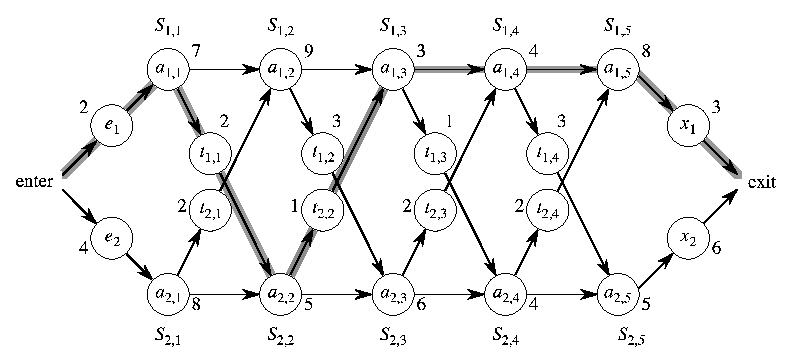
\includegraphics[scale=0.9]{assembly-line.eps}
}

\frame{
  \frametitle{Постановка задачи}
Задача: При всех заданных значениях $e_i, a_{i,j}, t_{i,j}, x_i$ определить самый быстрой способ
сборки одного шасси используя оба конвеера. \\
~\\
\pause
Перебором решить нельзя:
\begin{itemize}
\item Сущуествует $2^n$ возможных комбинаций. 
\item Неприемлимо при больших $n$.
\end{itemize}
}

\frame{
  \frametitle{Первый этап: структура оптимального решения}
  Подумаем о самом быстром пути от входа до <<за $S_{1,j}$>>:
  \begin{itemize}
    \item $j = 1$, просто: нужно только определить сколько времени
      займёт прохождение через $S_{1,1}$.
    \item $j \geq 2$, есть два варианта попасть к $S_{1,j}$:
      \begin{itemize}
        \item Через $S_{1,j-1}$, затем прямо в $S_{1,j}$.
        \item Через $S_{2,j-1}$, затем переместиться на другой конвеер
          и попасть в $S_{1,j}$.
      \end{itemize}
  \end{itemize}
  \pause
  Оптимальное решение задачи (самый быстрый путь через $S_{1,j}$) содержит в себе оптимальное решение
  подзадач (самый быстрый путь через $S_{1,j-1}$ или $S_{2,j-1}$). Это
  свойство назовём {\em оптимальной подструктурой}. 
}

\frame{
  \frametitle{Второй этап: рекурсивное решение}
  \begin{itemize}
    \item $f_i[j]$ --- самое быстрое время пройти этап $S_{i,j}$.
    \item Цель: найти самое быстрое время пройти все этапы конвеера,
      $f^*$:
      \[
      f^* = \min(f_1[n] + x_1, f_2[n] + x_2).
      \]
    \item В начале:
      \[
      \begin{split}
      f_1[1] &= e_1 + a_{1,1} \\
      f_2[1] &= e_2 + a_{2,1} \\
      \end{split}
      \]
    \item Для остальных $j=2, \ldots n$:
      \[
      \begin{split}
      f_1[j] &= \min(f_1[j-1] + a_{1,j}, f_2[j-1]+t_{2,j-1}+a_{1,j}) \\
      f_2[j] &= \min(f_2[j-1] + a_{1,j}, f_1[j-1]+t_{1,j-1}+a_{2,j}) 
      \end{split}
      \]
  \end{itemize}
}

\frame{
  \frametitle{Сохранение пути}
  $f_i[j]$ сохраняет только оптимальное значение, восстановить по нему
  путь сложно. Для упрощения введём дополнительный массив:
  \begin{itemize}
    \item $l_i[j]$ --- номер конвеера, откуда была пришёл на  $j$-ю
      позицию объект. 
    \item $l^*$ --- конвеер, на котором объект побывал в $n$-ой
      позиции. 
  \end{itemize}
}

\frame[plain]{
  \frametitle{Третий этап: вычисление минимальных промежутков времени}
  Можно было бы реализовать рекурсию и вычислить <<сверху вниз>>, однако это будет слишком
  долго. Введём значения $r_i(j)$ --- количество обращений к величине
  $f_i[j]$ в рекурсивном алгоритме. Тогда:
  \begin{itemize}
  \item $r_1(n) = r_2(n) = 1$.
  \item $r_1(j) = r_2(j) = r_1(j+1) + r_2(j+1)$ для $j=1,\ldots,
    n-1$. Покажем, что $r_i(j) = 2^{n-j}$:
    \begin{enumerate}
      \item $j=n$, тогда $2^{n-j}=2^0 = 1 = r_i(n)$.
      \item Предположим, что $r_i(j+1) = 2^{n-(j+1)}$, тогда:
        \[
        \begin{split}
          r_i{j} &= r_i(j+1) + r_2(j+1) \\
          &= 2^{n-(j+1)} + 2^{n-(j+1)} \\
          &= 2^{n-(j+1)_1} = 2^{n-j}
        \end{split}
        \]
    \end{enumerate}
  \item Т.е., значение $f_1[1]$ будет вычислено $2^{n-1}$ раз!
  \end{itemize}
}

\frame{
  \frametitle{Вычисление <<снизу вверх>>}
  \begin{itemize}
    \item $f_i[j]$ зависит только от $f_1[j-1]$ и $f_2[j-1]$ для
      $j\geq 2$.
    \item Нужно вычислять в порядке возрастания $j$.
  \end{itemize}
}

\frame{
  \frametitle{Алгоритм вычисления минимального времени}
  \begin{codebox}
    \li $f_1[1] \gets e_1+a_{1,1}$, $f_2[1] \gets e_2 + a_{2,1}$
    \li \For $j\gets 2$ \To $n$ \Do
    \li \If $f_1[j-1] + a_{1,j} \leq f_2[j-1] + t_{2,j-1} + a_{1,j}$
    \li \Then $f_1[j] \gets f_1[j-1]+a_{1,j}$, $l_1[j] \gets 1$
    \li \Else $f_1[j] \gets f_2[j-1]+t_{2,j-1}+a_{1,j}$, $l_1[j] \gets
    2$ \End
    \li \If $f_2[j-1] + a_{2,j} \leq f_1[j-1] + t_{1,j-1} + a_{2,j}$
    \li \Then $f_2[j] \gets f_2[j-1]+a_{2,j}$, $l_2[j] \gets 2$
    \li \Else $f_2[j] \gets f_1[j-1]+t_{1,j-1}+a_{2,j}$, $l_2[j] \gets
    1$ \End
    \End
    \li \If $f_1[n] + x_1 \leq f_2[n] + x_2$
    \li \Then $f^*\gets f_1[n]+x_1$, $l^* \gets 1$
    \li \Else $f^*\gets f_2[n]+x_2$, $l^* \gets 2$
    \End
  \end{codebox}
  
}

\frame[plain]{
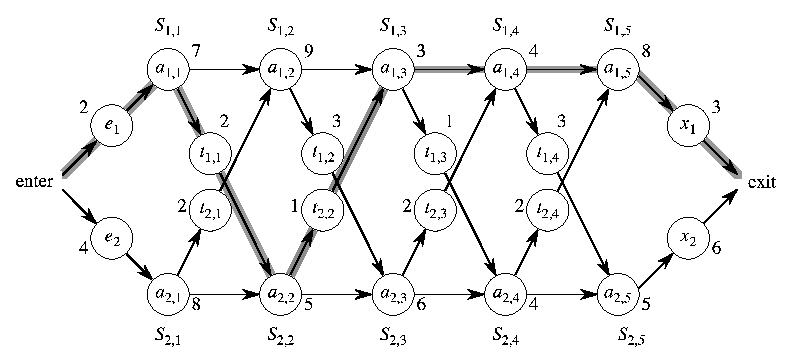
\includegraphics[scale=0.9]{assembly-line.eps}\\
~\\
~\\
\begin{columns}
\begin{column}{.5\textwidth}
\begin{tabular}{r|ccccc}
$j$ & 1 & 2 & 3 & 4 & 5 \\
\hline
$f_1[j]$ & 9 & 18 & 20 & 24 & 32 \\
$f_2[j]$ & 12 & 16 & 22 & 25 & 30 
\end{tabular}\\
\[
f^* = 35
\]
\end{column}
\begin{column}{.5\textwidth}
\begin{tabular}{r|cccc}
$j$ & 2 & 3 & 4 & 5 \\
\hline
$l_1[j]$ & 1 & 2 & 1 & 1 \\
$l_2[j]$ & 1 & 2 & 1 & 2 
\end{tabular}\\
\[
l^* = 1
\]
\end{column}
\end{columns}
}


\frame{
  \frametitle{Четвёртый этап: построение самого быстрого пути}
  \begin{codebox}
    \li $i \gets l^*$
    \li \id{print} <<Конвейер $i$, рабочее место $n$>>
    \li \For $j\gets n$ \Downto 2 \Do
    \li $i \gets l_i[j]$
    \li \id{print} <<Конвейер $i$, рабочее место $j-1$>>
    \End
  \end{codebox}
}


\subsection{Перемножение цепочки матриц}

\frame{
  \frametitle{Задача}
  Имеется последовательность (цепочка), состоящая из $n$ матриц, нужно
  вычислить их произведение:
  \[
  A_1A_2\cdots A_n.
  \]
  Для $\langle A_1, A_2, A_3, A_4 \rangle$ есть пять вариантов вычисления произведения:
  \[
  \begin{array}{c}
    (A_1(A_2(A_3A_4))), \\
    (A_1((A_2A_3)A_4)), \\
    ((A_1A_2)(A_3A_4)), \\
    ((A_1(A_2A_3))A_4), \\
    (((A_1A_2)A_3)A_4).
  \end{array}
  \]
}

\frame{
  \frametitle{Перемножение матриц}
  \begin{codebox}
    \li \If $\id{columns}[A] \neq \id{rows}[B]$ 
    \li \Then \Error <<Несовместимые размеры>>
    \li \Else \For $i \gets 1$ \To $\id{rows}[A]$ \Do
    \li \For $j \gets 1$ \To $\id{columns}[B]$ \Do
    \li $C[i,j] \gets 0$
    \li \For $k \gets 1$ \To $\id{columns}[A]$ \Do
    \li $C[i,j] \gets C[i,j] + A[i,k]\cdot B[k,j]$ \End \End \End
    \li \Return $C$ \End 
  \end{codebox}
  \begin{itemize}
    \item $A_{p\times q}\times B_{q \times r} = C_{p\times r}$.
    \item Время вычислений определяется количеством произведений
      скаляров, $pqr$.
  \end{itemize}
}

\frame{
  \frametitle{Стоимость перемножения матриц}
  
  \begin{itemize}
  \item Три матрицы $\langle A_1, A_2, A_3 \rangle$ размерностями $10
    \times 100$, $100 \times 5$ и $5 \times 50$.
  \item Перемножение $((A_1A_2)A_3)$ потребует сначала $10\cdot 100 \cdot
    500=2500$ скалярных произведений, а затем ещё $10\cdot 5 \cdot
    50=2500$,  т.е. всего $7500$ произведений. 
  \item Для вычисления $(A_1(A_2A_3))$ потребуется $100\cdot 5 \cdot
    50=25000$ скалярных умножений и ещё $10 \cdot 100 \cdot 50=50000$
    скалярных умножений, т.е. всего $75000$.
  \end{itemize}
}

\frame{
  \frametitle{Постановка задачи}
  Для заданной последовательности матриц $\langle A_1, A_2, \ldots,
  A_n \rangle$, в которой матрица $A_i$ имеет размер $p_{i-1}\times
  p_i$, с помощью скобок следует полностью определить порядок
  умножений в матричном произведении $A_1A_2\cdots A_n$, при котором
  количество скалярных умножений сведётся к минимуму. 
}

\frame{
  \frametitle{Перебор?}
  $P(n)$ --- количество альтернативных способов расстановки скобок в
  последовательности матриц:
  \[
  P(n) = \left\{ \begin{array}{ll}
        1 & \text{при } n=1 \\
        \displaystyle\sum_{k=1}^{n-1}P(k)P(n-k) & \text{при } n\geq 2
      \end{array}\right.
  \]

  $P(n) = \Omega(4^n/n^{3/2})$,  т.е. количество вариантов расстановки
  скобок экспоненциально увеличивается с ростом $n$ и метод прямого
  перебора не подходит. 
}

\frame{
  \frametitle{Первый этап: структура решения}

  \begin{itemize}
  \item $A_{i\ldots j} = A_iA_{i+1}\cdots A_j$, где $i \leq j$.
  \item Если $i < j$, то $i \leq k < j$ соответствует расстановка
    скобок: 
\[
A_{i\ldots j} = (A_{i\ldots k})\cdot(A_{k+1 \ldots j})
\]
\item Стоимость расстановки скобок будет равна сумме {\em оптимальной}
  стоимости перемножения $A_{i\ldots k}$, {\em оптимальной} стоимости
  $A_{k+1 \ldots j}$ и стоимости вычисления их произведения.
  \item Задача разбивается на две подзадачи и строится из оптимальных
    решений подзадач. 
 
  \end{itemize}
}

\frame{
  \frametitle{Второй этап: рекурсивное решение}
  $m[i,j]$ --- минимальное количество скалярных умножений, необходимых
  для вычисления матрицы $A_{i\ldots j}$. Тогда:
  \[
  m[i,j] = \left\{
      \begin{array}{ll}
        0 & \text{при } i=j,\\
        \displaystyle\min_{i\leq k < j}\left\{m[i,k] + m[k+1,j] +
        p_{i-1}p_kp_j \right\} & \text{при } i<j.
      \end{array}
      \right.
  \]
}

\frame{
  \frametitle{Третий этап: вычисление оптимальной стоимости}
  \begin{codebox}
    \Procname{$\proc{Matrix-Chain-Order}(p)$} 
    \li $n \gets \id{length}[p]-1$
    \li \For $i \gets 1$ \To $n$ \Do
    \li $m[i,i] \gets 0$ \End
    \li \For $l \gets 2$ \To $n$ \Do
    \li \For $i \gets 1$ \To $n-l+1$ \Do
    \li $j \gets i+l-1$, $m[i,j] \gets \infty$
    \li \For $k \gets i$ \To $j-1$ \Do
    \li $q \gets m[i,k] + m[k+1,j] + p_{i-1}p_kp_j$
    \li \If $q < m[i,j]$ 
    \li \Then $m[i,j] \gets q$ 
    \li \Else $m[i,j] \gets q$, $s[i,j] \gets k$ \End \End \End\End
    \li \Return $\langle m, s \rangle$
  \end{codebox}
}

\frame{
  \frametitle{Пример вычислений}
  \begin{columns}
    \begin{column}{.7\textwidth}
  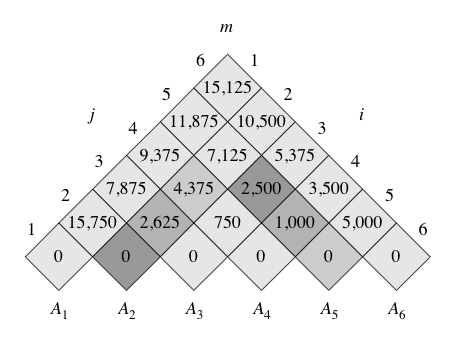
\includegraphics{matrix-chain-1.eps}
  \end{column}
  \begin{column}{.3\textwidth}
    \begin{tabular}{cc}
      $A_1$ & $30\times 35$ \\
      $A_2$ & $35\times 15$ \\
      $A_3$ & $15\times 5$ \\
      $A_4$ & $5\times 10$ \\
      $A_5$ & $10\times 20$ \\
      $A_6$ & $20\times 25$ \\
      \end{tabular}
    \end{column}
  \end{columns}
}

\frame{
  \frametitle{Массив $s$}
  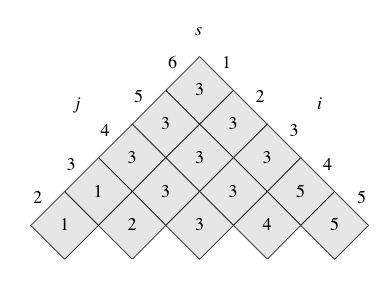
\includegraphics{matrix-chain-2.eps}
}

\frame{
  \frametitle{Четвёртый этап: получение решения}
  \begin{codebox}
    \Procname{$\proc{Print-Optimal-Parens}(s,i,j)$} 
    \li \If $i \isequal j$
    \li \Then \id{print} <<$A_i$>>
    \li \Else \id{print} <<(>>
    \li $\proc{Print-Optimal-Parens}(s,i,s[i,j])$
    \li $\proc{Print-Optimal-Parens}(s,s[i,j]+1,j)$
    \li \id{print} <<)>> \End
  \end{codebox}
}



\section{Элементы динамического программирования}
\frame{
  \frametitle{Применимость}
  Когда применим метод динамического программирования? 
  \begin{itemize}
    \item Оптимальная подструктура. 
    \item Перекрытие вспомогательных подзадач.
  \end{itemize}
}
\subsection{Оптимальная подструктура}

\frame{
  \frametitle{Оптимальная подструктура}
  \begin{itemize}
    \item Показывает, что решение задачи состоит из некоторого выбора,
      оставляющего одну или больше подзадач для решения. 
    \item Представим, что мы знаем последний выбор, который привёл к
      оптимальному решению. 
    \item Зная его, определим, какие подзадачи были возможны и выявим
      характеристики полученного пространства подзадач.
    \item Покажем, что решения подзадач для получения общего
      оптимального решения должны быть так же оптимальными. (обычно,
      от противного)
  \end{itemize}
}

\frame{
  \frametitle{Пространство подзадач}
  Нужно убедиться, что были рассмотрены все варианты выбора 
  подзадач. Однако:
  \begin{itemize}
    \item Нужно держать пространство подзадач как можно более
      простым. 
    \item Расширять его при необходимости. 
  \end{itemize}
}

\frame{
  \frametitle{Время работы алгоритма}
  Говоря просто, время работы зависит от общего количества подзадач
  умноженного на количество вариантов выбора. Например:
  \begin{itemize}
  \item Для конвеера: $\Theta(n)$ подзадач, 2 варианта выбора на каждой задаче,
    т.е. $\Theta(n)$ времени. 
  \item Расстановка скобок: $\Theta(n^2)$ подзадач, $O(n)$
    вариантов выбора внутри каждой подзадачи, $O(n^3)$ времени. 
  \end{itemize}
}

\frame{
  \frametitle{Решение снизу вверх}
  \begin{itemize}
    \item Сначала найти оптимальные решения для подзадач. 
    \item Затем выбрать те, которые нужно использовать в оптимальном
      решении для всей задачи. 
  \end{itemize}
  С жадными алгоритмами это не так. 
}

\frame{
  \frametitle{Наличие оптимальной структуры}
  Дан ориентированный граф $G=(V,E)$ и вершины $u,v \in V$.
  Две похожие задачи:
  \begin{itemize}
    \item Задача о кратчайшем невзвешенном пути. Нужно найти путь от
      вершины $u$ к вершине $v$, состоящий из минимального количества
      рёбер.
    \item Задача о самом длинном невзвешенном пути. Определить простой
      (без циклов)
      путь от вершины $u$ к вершине $v$, состоящий из максимального
      количества рёбер, $u \leadsto v$.
  \end{itemize}
}

\frame{
  \frametitle{Оптимальная подструктура для кратчайшего пути}
  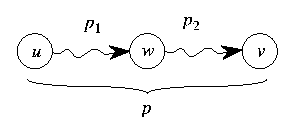
\includegraphics{shortest-path.eps}
  \begin{itemize}
    \item Допустим $p$ --- кратчайший путь $u \leadsto v$.
    \item $w$ --- любая вершина на $p$.
    \item $p_1$ --- подпуть $p$, $u \leadsto w$.
    \item Тогда $p_1$ --- кратчайший путь $u \leadsto w$.
    \item Допустим, существует более короткий путь, $p'_1$, $u
      \leadsto w$. Заменим в $p$  путь  $p_1$ на $p'_1$, получим путь
      $u \overset{p'_1}{\leadsto} w \overset{p_2}{\leadsto} v$ короче, чем $p$.
  \end{itemize}
}

\frame{
  \frametitle{Оптимальная подструктура для самого длинного пути}
  \begin{wrapfigure}{r}{.3\textwidth}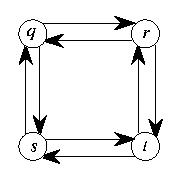
\includegraphics{longest-path.eps}\end{wrapfigure}
  Здача выглядит похоже, вероятно так же можно найти оптимальную
  подструктуру. Однако, это не так.
%  \begin{wrapfigure}{r}{.3\textwidth}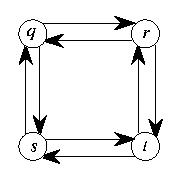
\includegraphics{longest-path.eps}\end{wrapfigure}
  \begin{itemize}
    \item $q \rightarrow r \rightarrow t$ --- самый длинный простой
      путь $q \leadsto t$. Но его подпути не являются самыми длинными
      путями!
    \item Подпуть для $q \leadsto r$: $q \rightarrow r$.  Самый
      длинный путь $q \rightarrow s \rightarrow t \rightarrow r$.
      \item Подпуть для $r \leadsto t$: $r \rightarrow t$. Самый
        длинный путь $r \rightarrow q \rightarrow s \rightarrow t$.
      \item  Комбинация самых длинных путей не является простым путём:
        $q \rightarrow s \rightarrow t \rightarrow r \rightarrow q
        \rightarrow s \rightarrow t$
     
  \end{itemize}
  
}

\frame{
  \frametitle{В чём отличие?}
  \begin{itemize}
  \item Задача о коротком пути имеет независимые подзадачи,
    т.е. решение одной позадачи не сказывается на решении другой
    подзадачи. 
  \item В задаче о длинном пути подзадачи зависимы. 
  \end{itemize}
}

\subsection{Перекрытие вспомогательных подзадач}

\frame{
  \frametitle{Неперекрывающиеся подзадачи}
  
  Хороший алгоритм вида <<разделяй-и-властвуй>> должен на каждом шаге
  решать совершенно новую подзадачу. Например, сортировка слиянием:
\begin{figure}
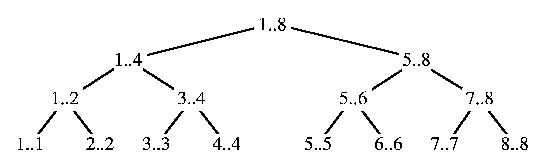
\includegraphics{merge-sort.eps}
\end{figure}
}

\frame{
  \frametitle{Перекрывающиеся подзадачи}
  \begin{itemize}
    \item Эффективность алгоритмов динамического программирования зависит от
  того, насколько часто одна и та же подзадача рассматривается в
  рекурсивном решении. 
  \item Перекрытие подазадач и независимость решения подзадач ---
    разные понятия!
  \item Если есть перекрытие, то можно либо выстроить
    эффективную последовательность решения подзадач, или
    модифицировать рекурсивный алгоритм, чтобы он запоминал
    промежуточные результаты. 
  \end{itemize}
}

\frame{
  \frametitle{Перекрытие в рекурсивном алгоритме}
  \begin{codebox}
    \Procname{$\proc{Recursive-Matrix-Chain}(p,i,j)$} 
    \li \If $i \isequal j$
    \li \Then \Return 0 \End
    \li $m[i,j] \gets \infty$
    \li \For $k \gets i$ \To $j-1$ \Do
    \li $q \gets \proc{Recursive-Matrix-Chain}(p,i,k)$
    \zi $+\proc{Recursive-Matrix-Chain}(p,k+1,j) + p_{i-1}p_kp_j$
    \li \If $q < m[i,j]$
    \li \Then $m[i,j] \gets q$ \End\End
    \li \Return $m[i,j]$
  \end{codebox}
}

\frame{
  \frametitle{Дерево рекурсии для (1,4)}
  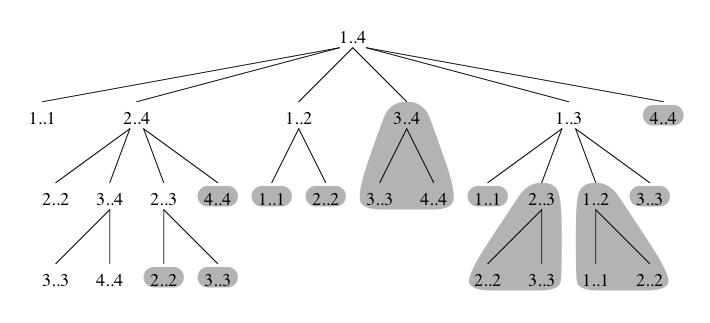
\includegraphics{matrix-chain-recursive.eps}
}

\frame[plain]{
  \frametitle{Запоминание}
    \begin{codebox}
    \Procname{$\proc{Memoized-Matrix-Chain}(p)$} 
    \li $n \gets \id{length}[p]-1$
    \li \For $i \gets 1$ \To $n$ \Do
    \li \For $j \gets i$ \To $n$ \Do
    \li $m[i,j] \gets \infty$ \End\End
    \li \Return $\proc{Lookup-Chain}(p,1,n)$
  \end{codebox}
  \begin{codebox}
    \Procname{$\proc{Lookup-Chain}(p,i,j)$} 
    \li \If $m[i,j] < \infty$
    \li \Then \Return $m[i,j]$ \End
    \li \If $i \isequal j$
    \li \Then \Return 0 \End
    \li \For $k \gets i$ \To $j-1$ \Do
    \li $q \gets \proc{Lookup-Chain}(p,i,k)+\proc{L-C}(p,k+1,j) + p_{i-1}p_kp_j$
    \li \If $q < m[i,j]$
    \li \Then $m[i,j] \gets q$ \End\End
    \li \Return $m[i,j]$
  \end{codebox}
}

\section{Ещё примеры}
\subsection{Самая длинная общая подпоследовательность}

\frame{
  \frametitle{Постановка задачи}
  Даны две последовательности, $X=\langle x_1, \ldots, x_m \rangle$ и
  $Y=\langle y_1, \ldots, y_n \rangle$. Нужно найти
  общую для обеих последовательностей подпоследовательность, чья длина
  будет наибольшей. \\
  ~\\
  Задача тесно связана с вычислением расстояния Левенштейна. 
}

\frame{
  \frametitle{Примеры}
  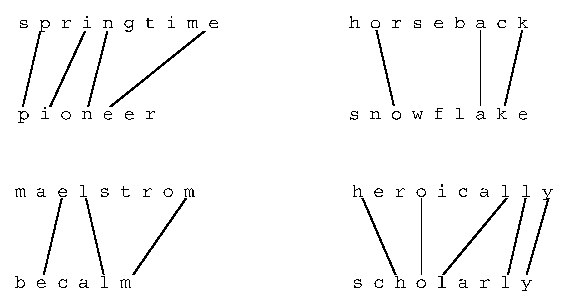
\includegraphics{lcs-ex.eps}
}

\frame{
  \frametitle{Перебор}
   Время на перебор $\Theta(n2^m)$:
   \begin{itemize}
   \item Нужно проверить $2^m$ подпоследовательностей $X$.
   \item Каждая проверка занимает $\Theta(n)$ времени. 
   \end{itemize}
}

\frame{
  \frametitle{Первый этап: оптимальная подструктура}
  Будем считать, что $X_i$ --- префикс $\langle x_1, \ldots, x_i
  \rangle$ и $Y_i$ --- префикс $\langle y_1, \ldots y_i \rangle$
  \begin{rtheorem}
    Пусть $Z=\langle z_1, \ldots z_k \rangle$ какая-то
    $LCS(X,Y)$. Тогда:
    \begin{enumerate}
    \item $x_m = y_n$, тогда $z_k = x_m = y_n$ и
      $Z_{k-1}=LCS(X_{m-1},Y_{m-1})$.
    \item $x_m \neq y_n$ и $z_k \neq x_m$, тогда $Z=LCS(X_{m-1},Y)$.
    \item $x_m \neq y_n$ и $z_k \neq y_n$, тогда $Z=LCS(X,Y_{n-1})$.
    \end{enumerate}
  \end{rtheorem}
}

\frame{
  \begin{proof}
    \begin{itemize}
      \item $x_m = y_n$, допустим $z_k \neq x_m$. Тогда возьмём
        $Z'=\langle z_1, \ldots, z_k, x_m \rangle$, которая будет
        являться подпоследовательностью $X$ и $Y$ длиной $k+1$, что
        невозможно. 
      \item $x_m \neq y_n$ и $z_k \neq x_m$. Тогда $Z$ --- общая
        подпоследовательность для $X_{m-1}$ и $Y$. И она наибольшая,
        потому что в противном случае должна была бы существовать
        $W=LCS(X_{m-1},Y)$ длиной большей $k$, которая была бы
        $LCS(X,Y)$ длиной большей $k$, что невозможно.
      \item $x_m \neq y_n$ и $z_k \neq y_n$ --- аналогично. 
    \end{itemize}
  \end{proof}
}

\frame{
  \frametitle{Второй этап: рекурсивное определние}

  $c[i,j]=|LCS(X_i,Y_j)|$, нам нужно вычислить $c[m,n]$. Тогда:

  \[
  c[i,j] = \left\{\begin{array}{ll}
0& i=0 \text{ или } j=0, \\
c[i-1,j-1]+1& i,j>0 \text{ и } x_i=y_j, \\
\max(c[i-1,j],c[i,j-1])& i,j>0 \text{ и }x_i \neq y_j.
\end{array}
\right.
  \]
}

% В картинке в правом поддереве написано 3,3, должно быть 4,2
%\frame{
%  \frametitle{Дерево рекурсии}
%  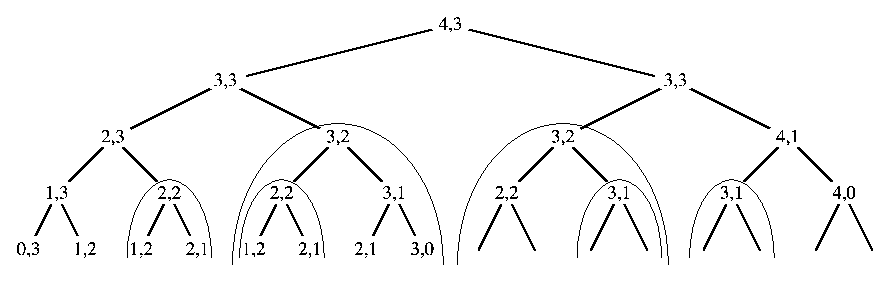
\includegraphics[scale=.8]{lcs-rec.eps}
  

%  Найдите ошибку.
%}

\frame{
  \frametitle{Третий этап: алгоритм}
  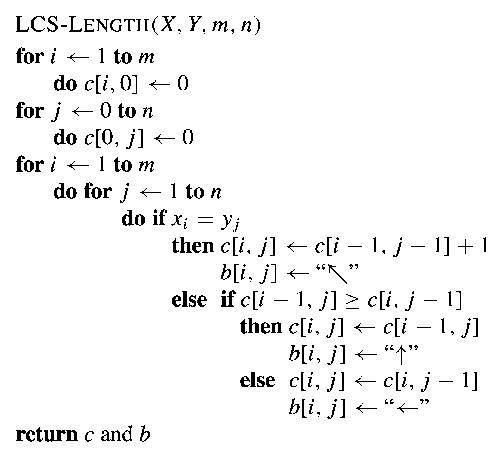
\includegraphics[scale=1]{lcs-alg.eps}
}

\frame{
  \frametitle{Четвёртый этап: распечатка решения}
  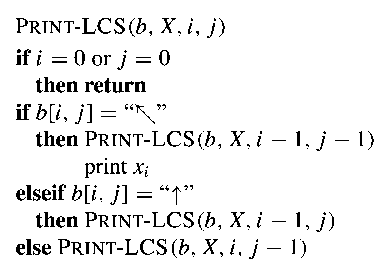
\includegraphics[scale=1]{lcs-print.eps}
}

\frame[plain]{
  \frametitle{Пример}
  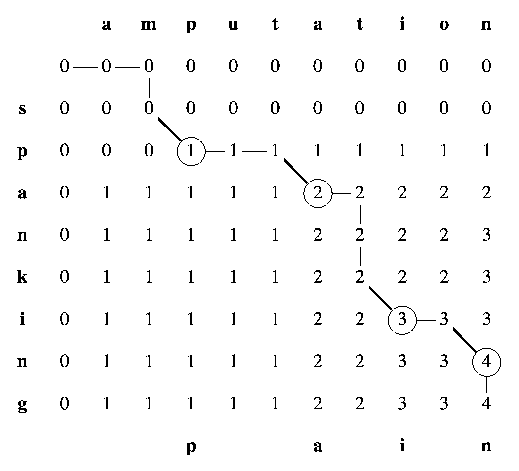
\includegraphics[scale=1]{lcs-example.eps}
}

\subsection{Оптимальные деревья поиска}

\frame{
  \frametitle{Постановка задачи}
  \begin{itemize}
  \item $n$ отсортированных различных ключей: $K=\langle k_1, k_2,
    \ldots, k_n \rangle$. 
  \item  $p_i$ --- вероятность поиска ключа $k_i$. 
  \item Вероятность поиска отсутствующих значений: 
    \begin{itemize}
      \item $n+1$ фиктивных ключей $\langle d_0, d_1, \ldots, d_n
        \rangle$, $d_0 < k_1$, $k_i < d_i < k_{i+1}$ ($1 \leq i < n$),
        $k_n < d_n$.
      \item $q_i$ --- вероятность поиска ключей, соответствующих
        $d_i$. 
    \end{itemize}
  \item  Поиск может быть успешным или неуспешным, т.е.:
\[
\sum_{i=1}^n p_i + \sum_{i=0}^nq_i = 1.
\]
  \end{itemize}
}

\frame{
  \frametitle{Стоимость поиска}
  \[
  \begin{split}
  \mathrm{E}[\mathrm{COST}(T)] &=
  \sum_{i=1}^n(depth_T(k_i)+1)\cdot p_i 
  + \sum_{i=0}^n(depth_T(d_i)+1)\cdot q_i \\
   &= 1 + \sum_{i=1}^n depth_T(k_i)\cdot p_i + \sum_{i=0}^n
   depth_T(d_i)\cdot q_i
  \end{split}
  \]
  \pause
  Нужно для данного набора вероятностей построить бинарное дерево
  поиска, математическое ожиданеие стоимости поиска для которого будет
  минимальным. Такое дерево --- оптимальное бинарное дерево поиска. 
}

\frame{
  \frametitle{Сбалансированное дерево поиска}
  \begin{tabular}{r|cccccc}
    $i$ & 0 & 1 & 2& 3& 4 & 5 \\
    \hline
    $p_i$ & & 0{,}15 & 0{,}10 & 0{,}05 & 0{,}10 & 0{,}20 \\
    $q_i$ & 0{,}05 & 0{,}10 & 0{,}05 & 0{,}05 & 0{,}05 & 0{,}10
  \end{tabular}
~\\
~\\
~\\
\begin{columns}
\begin{column}{.7\textwidth}
  \pstree[levelsep=30pt]{\Tcircle{$k_2$}}{
    \pstree{\Tcircle{$k_1$}}{
      \Tr{\psframebox{$d_0$}}
      \Tr{\psframebox{$d_1$}}
    }
    \pstree{\Tcircle{$k_4$}}{
      \pstree{\Tcircle{$k_3$}}{
        \Tr{\psframebox{$d_2$}}
        \Tr{\psframebox{$d_3$}}
      }
      \pstree{\Tcircle{$k_5$}}{
        \Tr{\psframebox{$d_4$}}
        \Tr{\psframebox{$d_5$}}
      }
    }
  }
\end{column}
\begin{column}{.3\textwidth}
  Стоимость дерева 2{.}80.
\end{column}
\end{columns}
}

\frame{
  \frametitle{Оптимальное дерево поиска}
  \begin{tabular}{r|cccccc}
    $i$ & 0 & 1 & 2& 3& 4 & 5 \\
    \hline
    $p_i$ & & 0{,}15 & 0{,}10 & 0{,}05 & 0{,}10 & 0{,}20 \\
    $q_i$ & 0{,}05 & 0{,}10 & 0{,}05 & 0{,}05 & 0{,}05 & 0{,}10
  \end{tabular}
~\\
~\\
~\\
\begin{columns}
\begin{column}{.5\textwidth}
  \pstree[levelsep=30pt]{\Tcircle{$k_2$}}{
    \pstree{\Tcircle{$k_1$}}{
      \Tr{\psframebox{$d_0$}}
      \Tr{\psframebox{$d_1$}}
    }
    \pstree{\Tcircle{$k_5$}}{
      \pstree{\Tcircle{$k_4$}}{
        \pstree{\Tcircle{$k_3$}}{
          \Tr{\psframebox{$d_2$}}
          \Tr{\psframebox{$d_3$}}
        }
        \Tr{\psframebox{$d_4$}}
      }
      \Tr{\psframebox{$d_5$}}
    }
  }
\end{column}
\begin{column}{.5\textwidth}
  \begin{enumerate}
  \item Стоимость дерева 2{.}75. 
  \item Оптимальное дерево может не быть идеально сбалансированным. 
  \item Ключ с
  максимальной вероятностью не обязан быть в корне.  
  \end{enumerate}
\end{column}
\end{columns}
}

\begin{frame}
  \frametitle{Перебор?}
  \begin{enumerate}
  \item Построить все деревья с $n$ узлами. 
  \item Рассчитать для каждого стоимость. 
  \item Выбрать оптимальное. 
  \end{enumerate}
  $\Omega(4^n/n^{3/2})$ различных бинарных деревьев с $n$
  узлами, поэтому перебор не подходит. 
\end{frame}

\begin{frame}
  \frametitle{Оптимальная подструктура}
  \begin{columns}
    \begin{column}{.6\textwidth}
      \begin{itemize}
        \item Поддерево бинарного дерева поиска содержит ключи из
          непрерывного диапазона $k_i, \ldots, k_j$ для $1 \leq i \leq
          j \leq n$.
        \item Если $T$ --- оптимальное дерево поиска и $T'$ --- его
          поддерево с ключами $k_i, \ldots, k_j$, то $T'$ должно быть
          оптимальным деревом с ключами $k_i,\ldots, k_j$ и фиктивными
          ключами $d_{i-1},\ldots, d_j$.
      \end{itemize}
    \end{column}
    \begin{column}{.4\textwidth}
      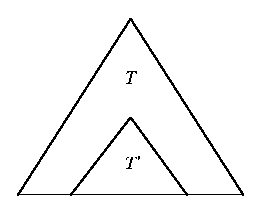
\includegraphics{bst-opt-subtree.eps}
    \end{column}
  \end{columns}
\end{frame}

\begin{frame}
  \frametitle{Выбор корня}
  \begin{columns}
    \begin{column}{.6\textwidth}
      \begin{itemize}
      \item Даны ключи $k_i, \ldots, k_j$ и $d_{i-1}, \ldots, d_j$. 
      \item Один из них, $k_r$, должен стать корнем. 
      \item Тогда левое поддерево состоит из $k_i, \ldots, k_{r-1}$ и
        $d_{i-1},\ldots, d_{r-1}$. 
      \item Правое поддерво --- из $k_{r+1}, \ldots, k_j$ и $d_r,
        \ldots, d_j$.
      \item Дерево из ключей $k_i, \ldots, k_{i-1}$ состоит из одного
        фиктивного ключа $d_{i-1}$.
      \end{itemize}
    \end{column}
    \begin{column}{.4\textwidth}
      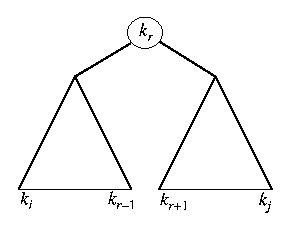
\includegraphics{bst-opt-div.eps}
    \end{column}
  \end{columns}
\end{frame}

\begin{frame}
  \frametitle{Рекурсивное решение}
  \begin{itemize}
  \item Задача поиска оптимального дерева, содержащего ключи $k_i, \ldots,
  k_j$, $i \geq 1$, $j \leq n$ и $j \geq i -1 $ (если $j=i-1$, то
  дерево состоит только из $d_{i-1}$. 
  \item $e[i,j]$ --- мат. ожидание
  стоимости поиска в дереве с ключами $k_i, \ldots, k_j$. 
  \item В конечном итоге, нужно
  вычислить $e[1,n]$
  \item В случае $j=i-1$ есть только $d_{i-1}$ и $e[i,i-1] = q_{i-1}$.
  \item  Если $j \geq i$, то среди ключей $k_i, \ldots, k_j$ нужно
    выбрать корень $k_r$ и составить левое и правое оптимальные
    деревья поиска из $k_i, \ldots, k_{r-1}$ и $k_{r+1},\ldots, k_j$.
\end{itemize}
\end{frame}

\begin{frame}
  Когда оптимальное дерево становится поддеревом, его стоимость
  увеличивается на 
  \[
  w(i,j) = \sum_{k=i}^j p_k + \sum_{k=i-1}^j q_k.
  \]
  Тогда:
  \[
  e[i,j] = p_r + (e[i,r-1] + w(i,r-1)) + (e[r+1,j] + w(r+1,j))
  \]
  Из 
  \[
  w(i,j) = w(i,r-1) + p_r + w(r+1,j)
  \]
  следует что:
  \[
  e[i,j] = e[i,r-1] + e[r+1,j] + w(i,j).
  \]
\end{frame}
\begin{frame}
  \frametitle{Точная запись решения}
  \[
  e[i,j] = \left\{
    \begin{array}{ll}
      q_{i-1} & j = i-1 \\
      \displaystyle\min_{i \leq r \leq j}\{e[i,r-1] + e[r+1,j] + w(i,j)\} & i \geq j
    \end{array}
    \right.
  \]
\end{frame}

\begin{frame}
  \frametitle{Алгоритм}
  \begin{codebox}
    \li \For $i \gets 1$ \To $n+1$ \Do
    \li $e[i,i-1] \gets q_{i-1}$, $w[,i-1] \gets q_{i-1}$ \End
    \li \For $k \gets 1$ \To $n$ \Do
    \li \For $j \gets 1$ \To $n-k+1$ \Do
    \li $j \gets i+k-1$, $e[i,j] \gets \infty$
    \li $w[i,j] \gets w[i,j-1] + p_j + q_j$
    \li \For $r \gets i$ \To $j$ \Do
    \li $t \gets e[i,r-1] + e[r+1,j] + w[i,j]$
    \li \If $t < e[i,j]$ 
    \li \Then $e[i,j] \gets t$, $root[i,j] \gets r$ \End
    \End \End \End
    \li \Return $\langle e, root \rangle$
  \end{codebox}
\end{frame}


%\subsection{Оптимальные бинарные деревья поиска}

\end{document}
    
